\documentclass[a4paper,10pt]{article}
\usepackage[margin=2.5cm]{geometry}
\usepackage[utf8]{inputenc}
\usepackage[colorlinks=true,urlcolor=blue]{hyperref}
\usepackage{amsmath}
\usepackage{graphicx}
\usepackage{float}
\usepackage{caption}
\usepackage{subcaption}
\usepackage{xcolor}
\usepackage{booktabs}

\usepackage{listings} %Alternative to minted
\definecolor{codegreen}{rgb}{0,0.6,0}
\definecolor{codegray}{rgb}{0.5,0.5,0.5}
\definecolor{codepurple}{rgb}{0.58,0,0.82}
\definecolor{backcolour}{rgb}{0.95,0.95,0.92}
 
\lstdefinestyle{mystyle}{
    backgroundcolor=\color{backcolour},   
    commentstyle=\color{codegreen},
    keywordstyle=\color{magenta},
    numberstyle=\tiny\color{codegray},
    stringstyle=\color{codepurple},
    basicstyle=\footnotesize,
    breakatwhitespace=false,         
    breaklines=true,                 
    captionpos=b,                    
    keepspaces=true,                 
    numbers=left,                    
    numbersep=5pt,                  
    showspaces=false,                
    showstringspaces=false,
    showtabs=false,                  
    tabsize=2
}

\lstset{style=mystyle}
\setlength{\parindent}{0em}
\setlength{\parskip}{1em}

\title{\textbf{Deep Learning for Image Analysis} 
\\ DL4IA -- Report for Assignment 3}
\author{Student Linus Falk}
\date{\today}

\begin{document}
\lstset{language=Python}
\maketitle

\section*{Introduction}
Third assignment in the course Deep learning for image analysis

\section{Classification of hand-written digits using a Convolutional
Neural Network}

\textit{\textbf{Exercise 1.1}}
In this exercise we implemented the same neural network as in assignment 2. But this time we used the PyTorch library and GPU support for training. The task was to compare the performance in accuracy and training time. The weight were initialized in the same way as in assignment 2 and training was done with the same hyperparameters, see table:\ref{tab:tab1}. As we can see in table \ref{tab:tab2} the accuracy performance is very similar since the architecture and the training methods is the same. The difference between the training times are on the other hand noticeably shorter for the PyTorch version. This is much thanks to the GPU support, but also more effective data handling then the "homeCooked" version has. In \ref{fig:a2torchver} we can see signs that the model is starting to overfit. The test loss has stopped to improve while the training loss on the subset (6000 samples) of the training set is still improving. The model is overfitting to the training data and if we would continue to train we would we decrease in performance on the test set. 

\begin{table}[ht!]
\centering
\begin{tabular}{ll}\hline
 \textbf{Hyperparameters}&    \\ \hline
 BatchSize&  30  \\
 Epochs&  60 \\ 
 lr& 0.01\\
Optimizer& SGD  \\\hline
\end{tabular}
\caption{example}
\label{tab:tab1}
\end{table}

\begin{figure}[ht!]
\centering
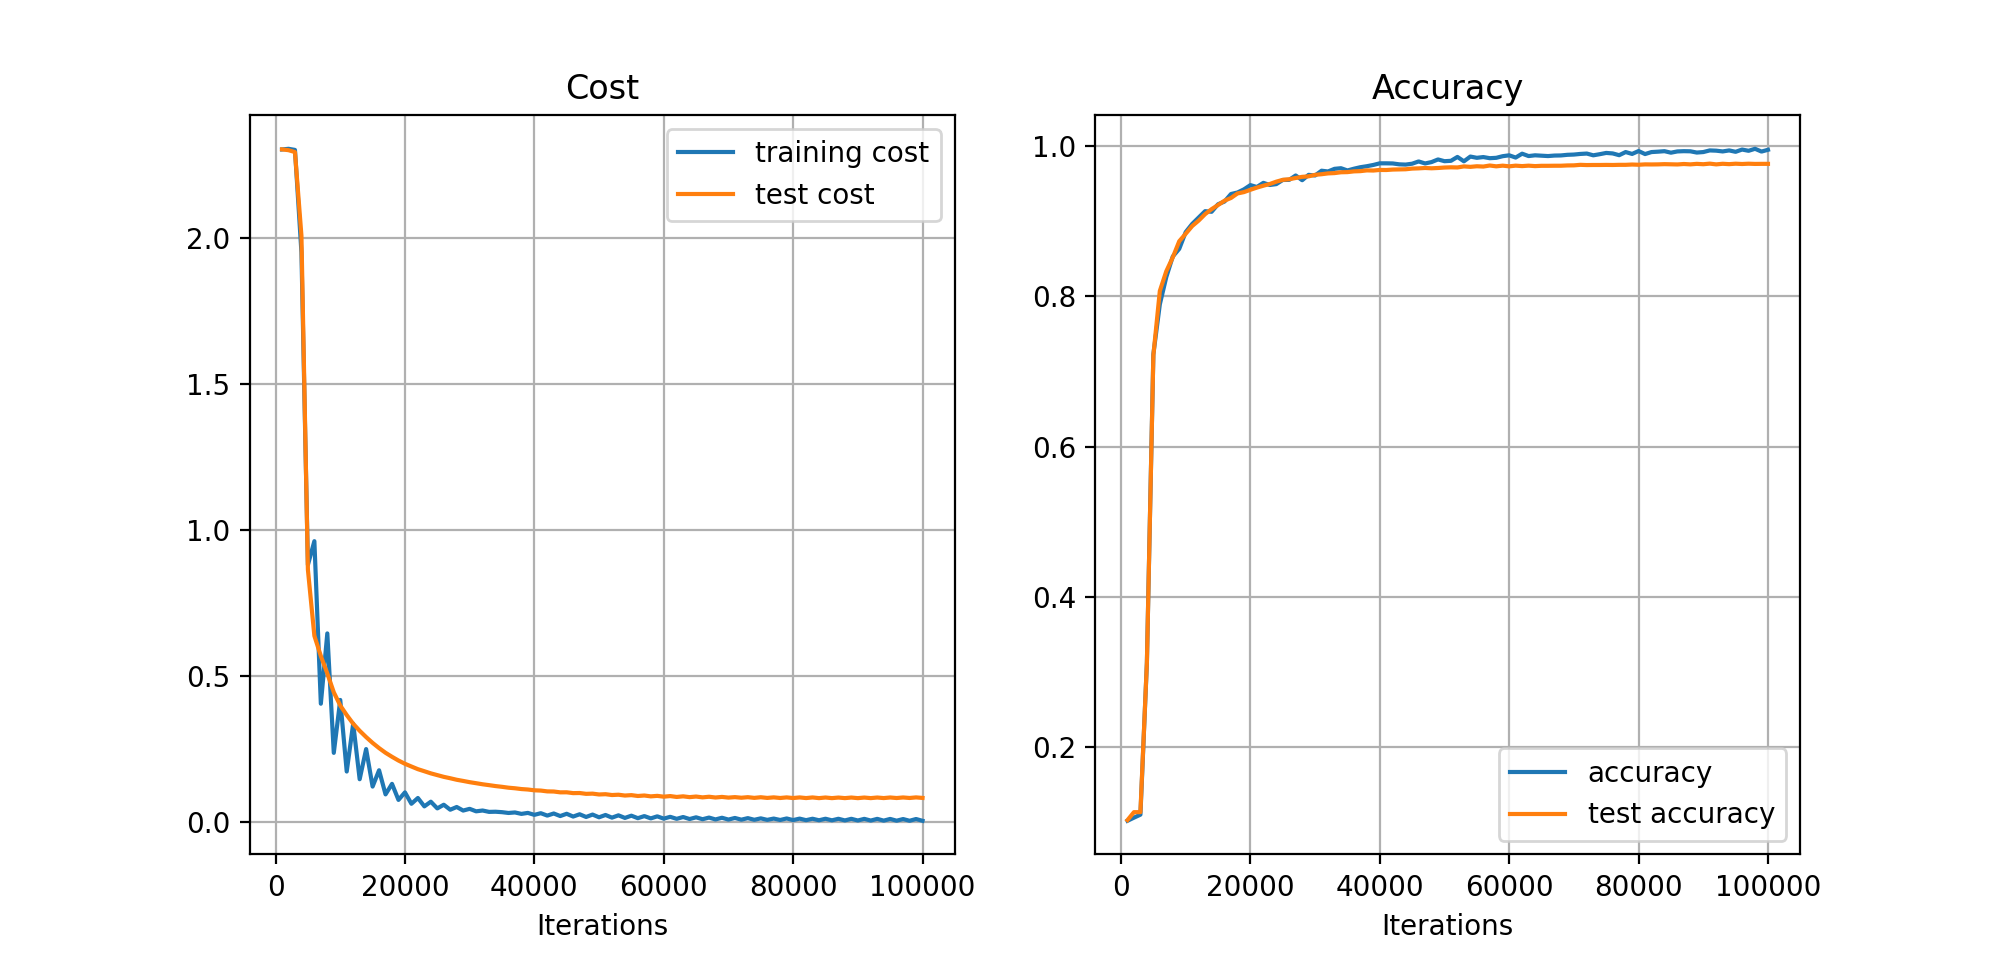
\includegraphics[width=120mm]{figures/assignment_3/A2_torchversion.png}
\caption{Training history: Assignment 2 Torch version, Accuracy: 97.22\%}
\label{fig:a2torchver}
\end{figure}


\begin{table}[ht!]
\centering
\begin{tabular}{lll}\hline
 &  \textbf{"HomeCooked NN"}& \textbf{PyTorch} \\ \hline
 Accuracy (\%) &  97.26&  97.22\\
 Time (sec)& 289 & 22.28\\ \hline
\end{tabular}
\caption{example}
\label{tab:tab2}
\end{table}


\newpage

\textit{\textbf{Exercise 1.2}}
In this exercise we construct a convolutional neural network with the PyTorch library according to the instructions. We compare the accuracy and number of weights between the Fully connected and the convolutional NN in table: \ref{tab:tab4}. Looking at the training history we can conclude that this network doesn't show the same signs of overfitting. The convolutional neural network has improved accuracy with fewer trainable weights. By using the CNN we improve the accuracy be preserving the spatial information and reduce the risk of overfitting by having fewer trainable parameters. 

\begin{table}[ht!]
\centering
\begin{tabular}{ll}\hline
 \textbf{Hyperparameters}&    \\ \hline
 BatchSize&  100  \\
 Epochs&  60 \\ 
 lr& 0.005 \\
Optimizer& SGD  \\\hline
\end{tabular}
\caption{example}
\label{tab:tab3}
\end{table}

\begin{figure}[ht!]
\centering
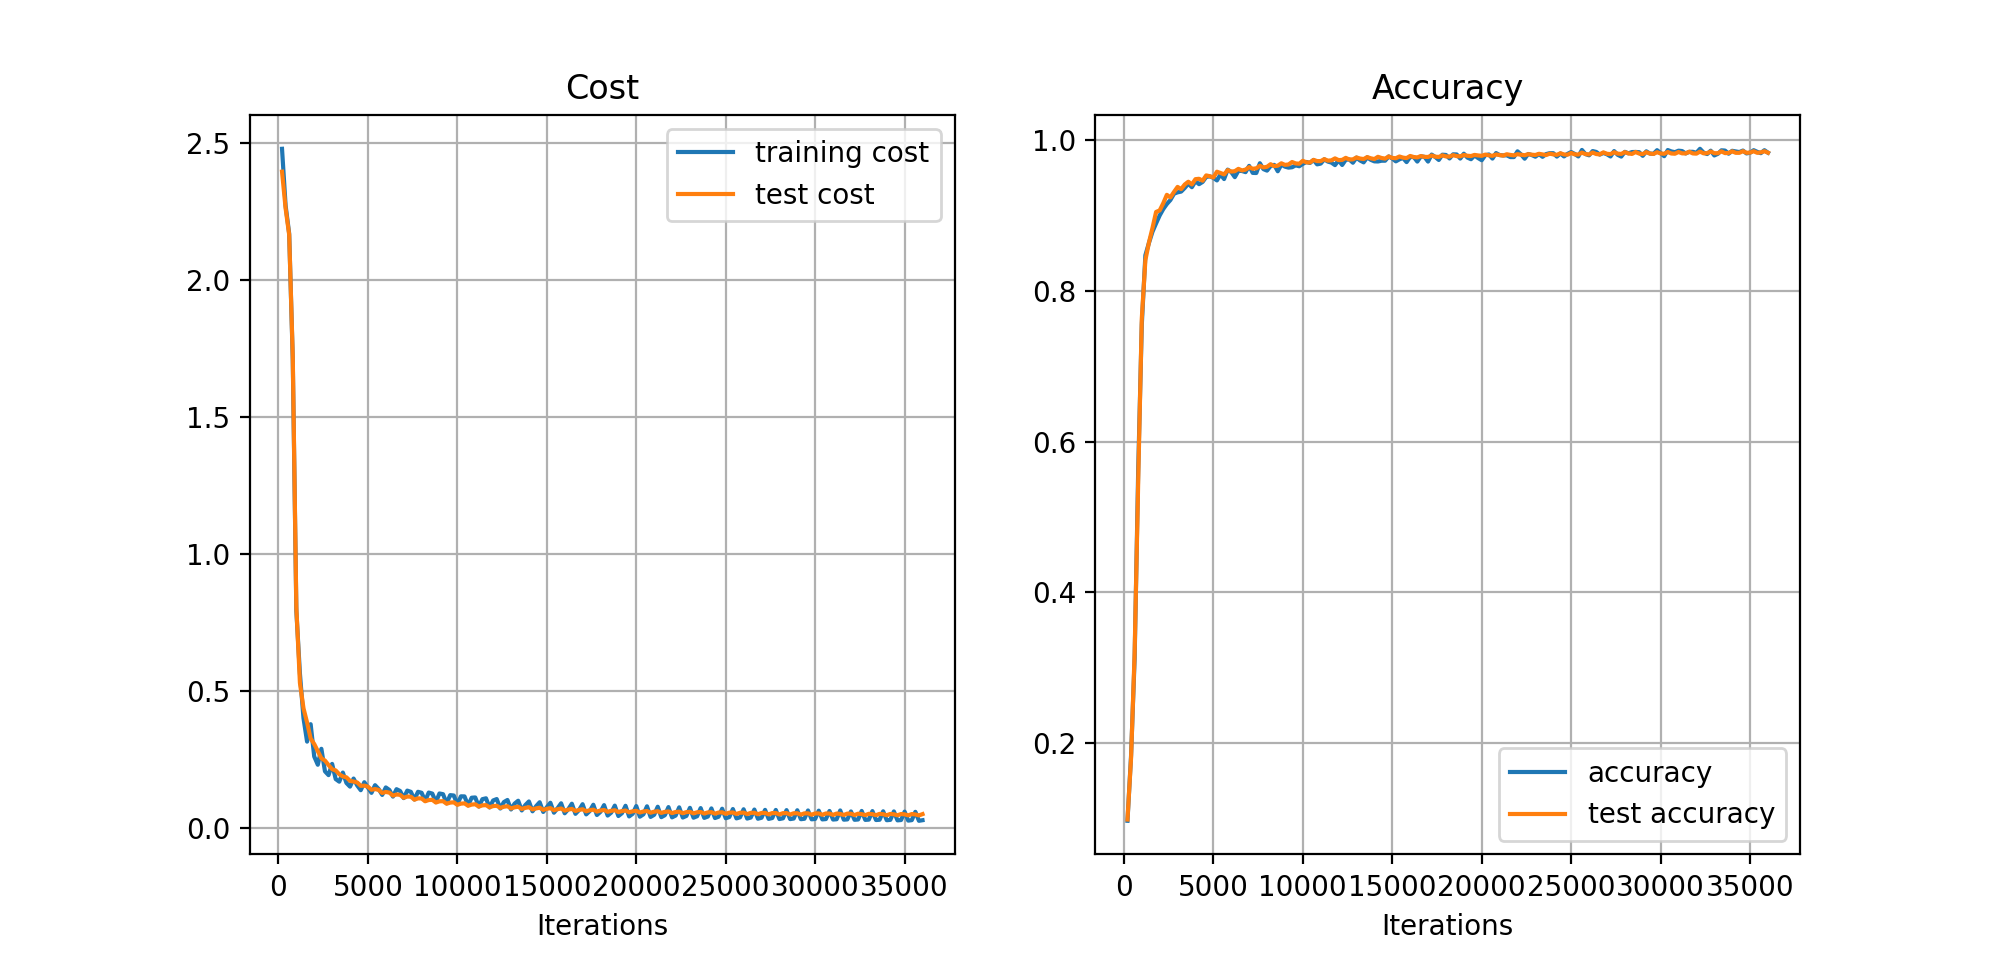
\includegraphics[width=120mm]{figures/assignment_3/convnet.png}
\caption{Training history Exercise 1.2, Accuracy: 98.35\%}
\label{fig:convnet1}
\end{figure}

\begin{table}[ht!]
\centering
\begin{tabular}{lll}\hline
 \textbf{Architecture}&  Accuracy (\%)& Number of weights  \\ \hline
 \textbf{FF}&  97.22&  109386\\ 
 \textbf{CNN}& 98.55& 21688 \\\hline
\end{tabular}
\caption{example}
\label{tab:tab4}
\end{table}

\newpage

\textit{\textbf{Exercise 1.3}} Here we are asked to swap place of the maxpooling layer and take the maxpooling before the activation function instead. This will result in fewer connections to the activation function making the time for calculating the activations fewer and therefore reducing the training time which we can see in: Table \ref{tab:tab5}. If we would use a more complicated activation function like the \emph{hyperbolic tangent} the time difference would increase. The worse accuracy in the swapped layer case can be caused by the fact that we are passing on less information to the activation function. 



\begin{table}[ht!]
\centering
\begin{tabular}{lll}\hline
 &  \textbf{CNN without swapped layers}& \textbf{CNN with swapped layers} \\ \hline
 Accuracy (\%) &98.55  &96.87  \\
 Time (sec)&  202& 135\\ \hline
\end{tabular}
\caption{Result Exercise 1.3}
\label{tab:tab5}
\end{table}

\begin{figure}[ht!]
\centering
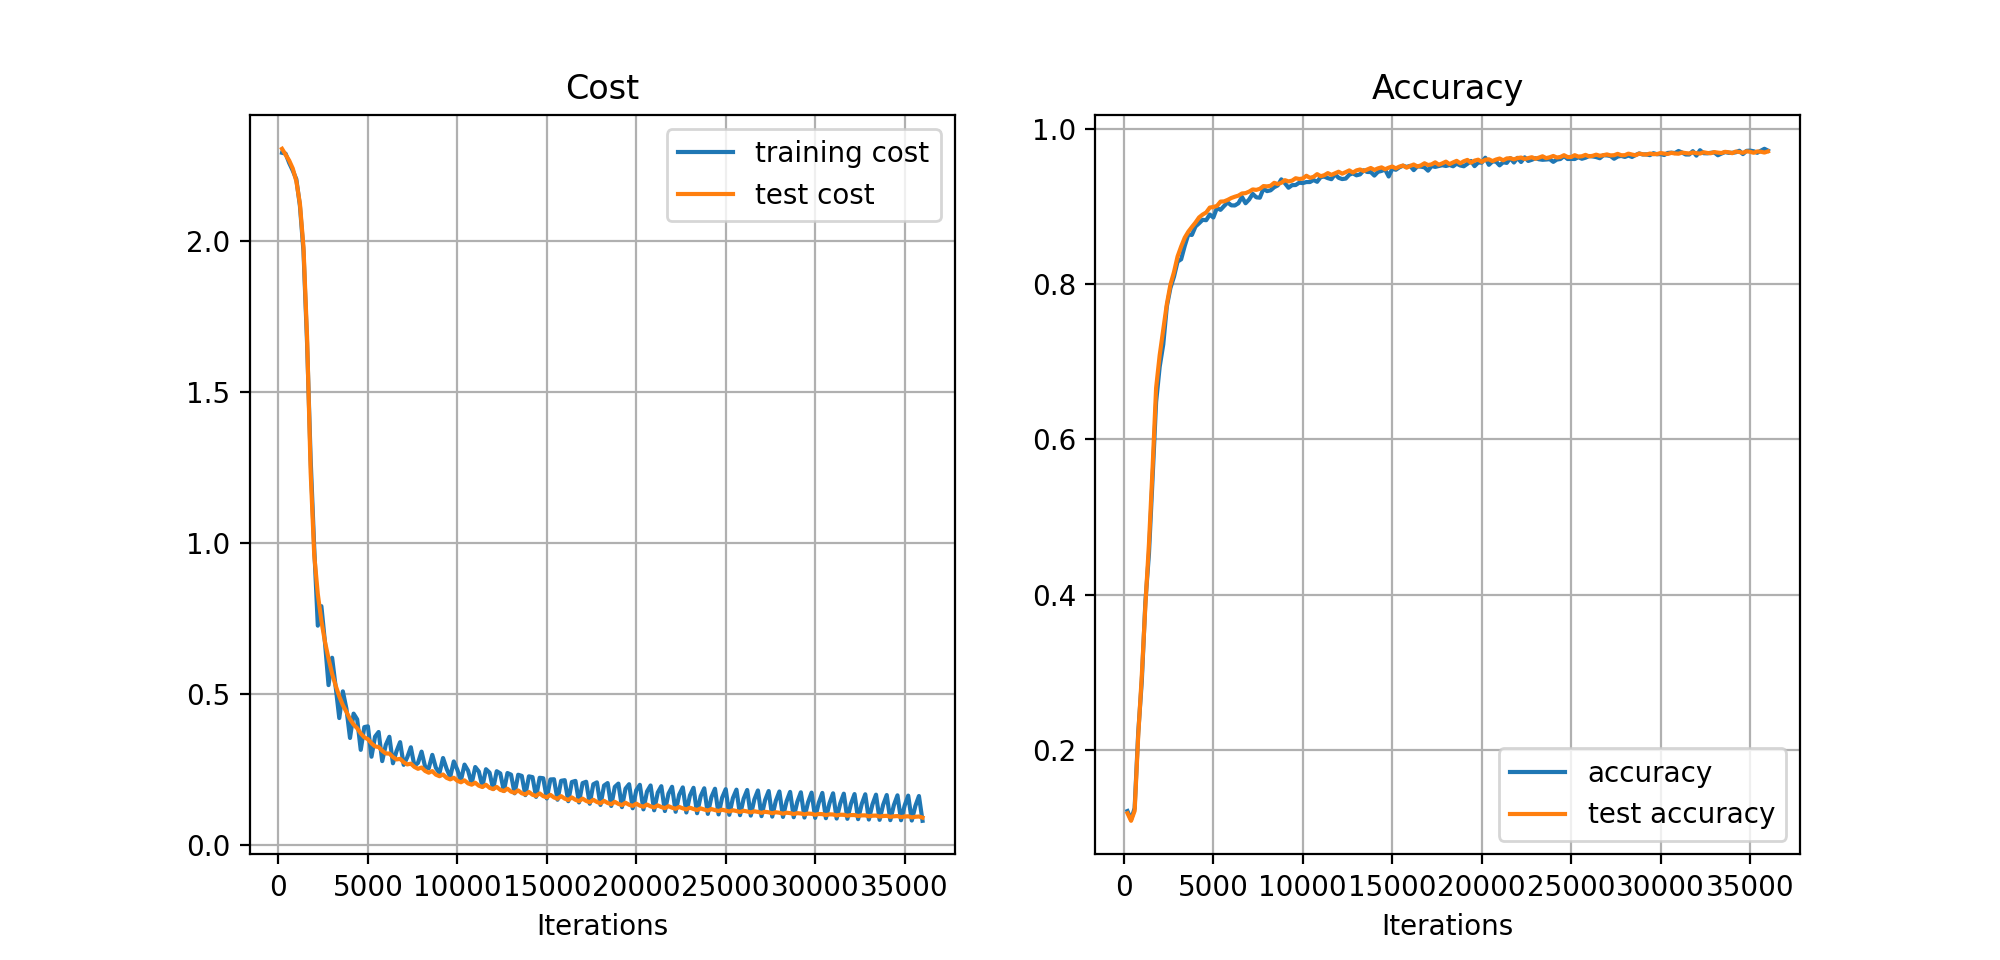
\includegraphics[width=120mm]{figures/assignment_3/convnet_swapped.png}
\caption{Training history Exercise 1.3}
\label{fig:example}
\end{figure}


\textit{\textbf{Exercise 1.4}} To investigate how the choice of optimizer effects the training time, we are here asked to use the optimizer: \emph{ADAM} (with default parameters) instead of \emph{SGD} and compare how much faster the training becomes.\emph{ADAM} is in many cases the best choice of optimizer and we can conclude from the result of our test in Table: \ref{tab:tab6} that we need fewer epochs to achieve the same (or better) accuracy as \emph{SGD} when using \emph{ADAM}. We can see that the training accuracy, in figure: \ref{fig:convnetadam} improving slightly more in the last iterations compared to the test set, indicating that were starting to get some overfitting.

\begin{table}[ht!]
\centering
\begin{tabular}{ll}\hline
 \textbf{Hyperparameters}&    \\ \hline
 BatchSize&  100  \\
 Epochs&  15 \\ 
 Optimizer& Adam  \\
 lr& 0.001 \\
 betas&  (0.9, 0.999) \\
 eps& 1e-8 \\
 weight\_decay& 0 \\ \hline
\end{tabular}
\caption{Hyperparameters Exercise 1.4}
\label{tab:tab3}
\end{table}

\begin{table}[ht!]
\centering
\begin{tabular}{lll}\hline
 &  \textbf{CNN trained with SGD}& \textbf{CNN trained with ADAM} \\ \hline
 Accuracy (\%) &98.55  & 98.69\\
 Time (sec)&  202& 73 \\ \hline
\end{tabular}
\caption{Result Exercise 1.4}
\label{tab:tab6}
\end{table}

\newpage

\begin{figure}[ht!]
\centering
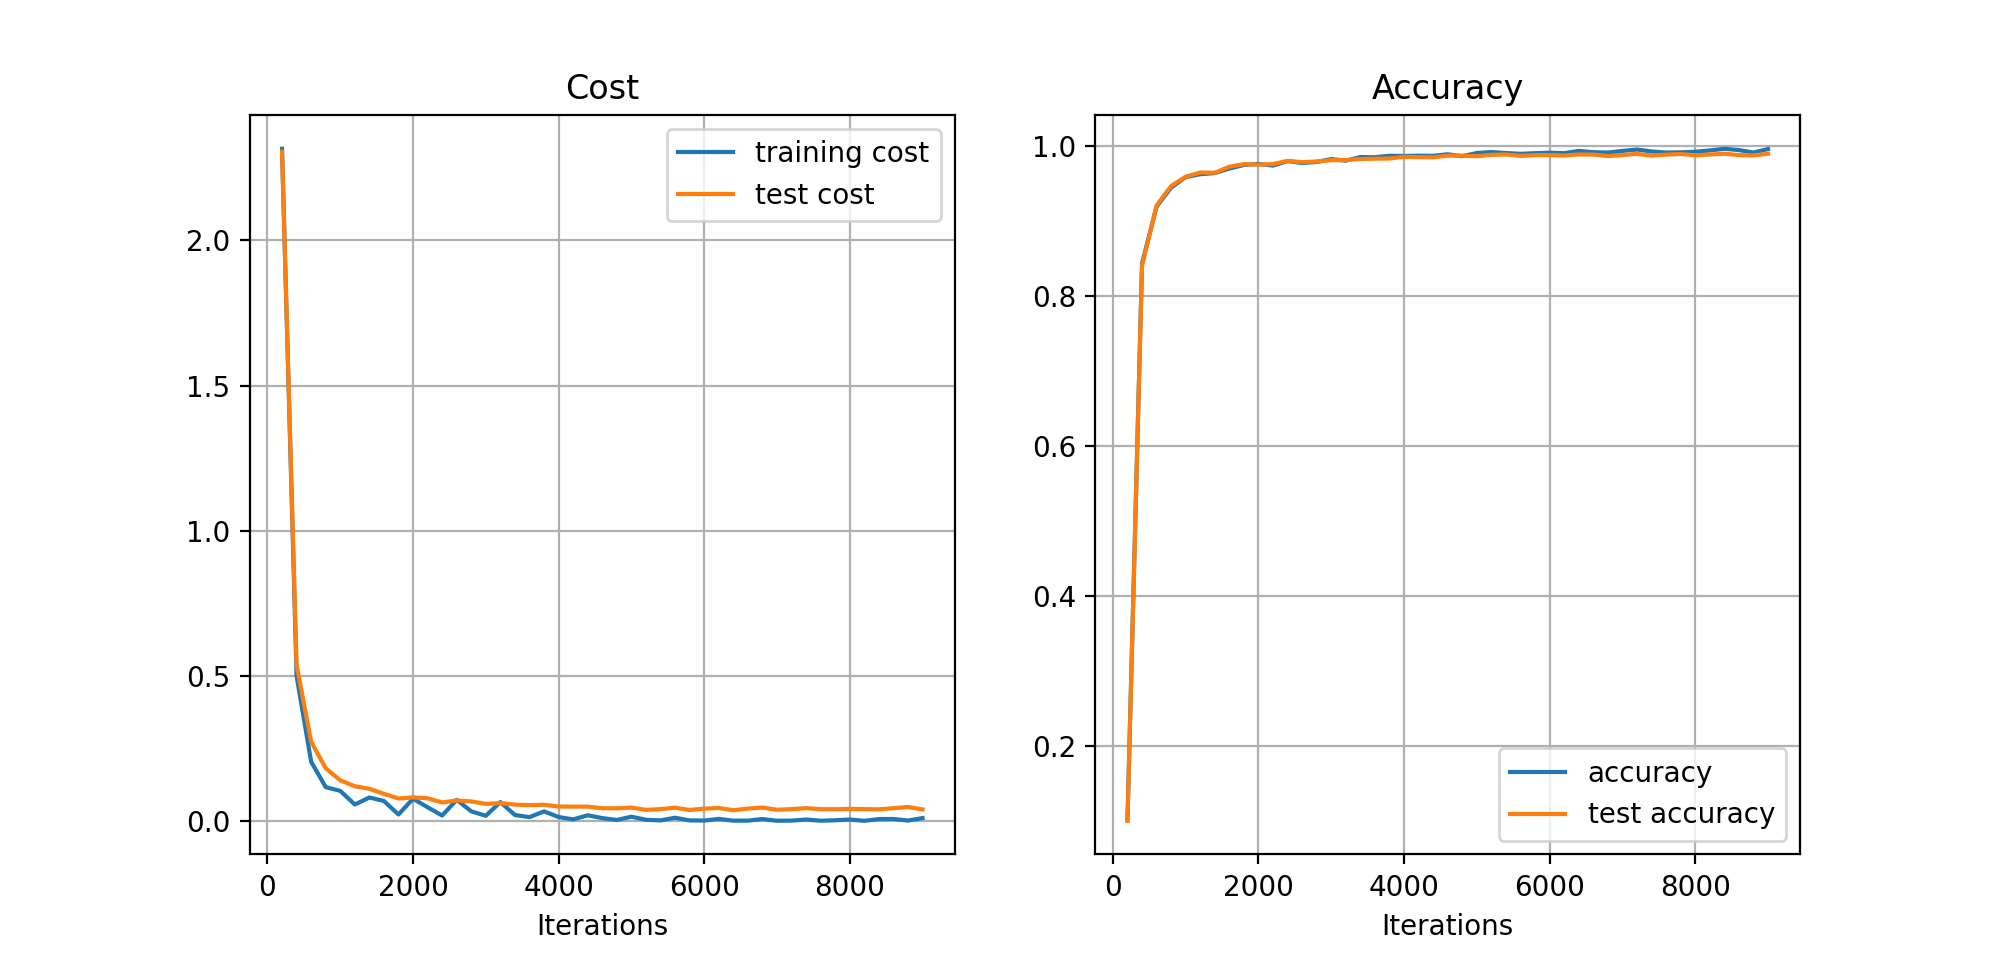
\includegraphics[width=120mm]{figures/assignment_3/convnet_adam.png}
\caption{Training history Exercise 1.3}
\label{fig:convnetadam}
\end{figure}


\textit{\textbf{Exercise 1.5}} In this exercise we try out at least 3 different ways to improve our model by changing for example architecture, learning rate or using different types of regularization methods. The result is presented below with tables of changes for each model and performance measure. The result from the best model is also presented with a confusion matrix of the test set. 

\textbf{Model 1:} We increase the last, fully connected layers to 50 nodes to improve see if we can improve the model with more learnable parameters. To reduce the risk of overfitting we also include a dropout layer after this layer with a probability, p=0,25. 
\begin{table}[ht!]
\centering
\begin{tabular}{ll}\hline
 \textbf{Hyperparameters}&    \\ \hline
 BatchSize&  100  \\
 Epochs&  10 \\ 
 Optimizer& Adam  \\
 lr& 0.003 \\ \hline
\textbf{Result: }&   98.8\% \\ \hline
\end{tabular}
\caption{Hyperparameters Exercise 1.5, Model 1}
\label{tab:tab7}
\end{table}

\textbf{Model 2:} Included batch normalization layers between all layers which can improve the training by normalizing all activation. In this case it didn't give major improvement since we didn't have a problem with vanishing or exploding gradients which it is most commonly used to improve. 

\begin{table}[ht!]
\centering
\begin{tabular}{ll}\hline
 \textbf{Hyperparameters}&    \\ \hline
 BatchSize&  100  \\
 Epochs&  10 \\ 
 Optimizer& Adam  \\
 lr& 0.003\\ \hline
\textbf{Result: }&   98.89\% \\ \hline
\end{tabular}
\caption{Hyperparameters Exercise 1.5, Model 2}
\label{tab:tab7}
\end{table}

\textbf{Model 3:} Here we change the learning rate strategy by changing the learning rate such that i depends on the iteration number (i) with the function:

    \begin{equation}
        \gamma^{(i)} = \gamma_{\text{min}} + (\gamma_{\text{max}} - \gamma_{\text{min}})e^{\frac{i} {2000} }
    \end{equation}

We set $\gamma_{\text{max}} = 0.003$ and $\gamma_{\text{min}} = 0.0001$ and update it throughout the training.

\begin{table}[ht!]
\centering
\begin{tabular}{ll}\hline
 \textbf{Hyperparameters}&    \\ \hline
 BatchSize&  100  \\
 Epochs&  10 \\ 
 Optimizer& Adam  \\
 lr& 0.003 - 0.0001 \\ \hline
\textbf{Result: }&   99.04\% \\ \hline
\end{tabular}
\caption{Hyperparameters Exercise 1.5, Model 3}
\label{tab:tab7}
\end{table}

\newpage

\textbf{Model 4:} Here we simply combine model 1 and model 3. Increasing the number of nodes to 200 in the final fully connected layer, add a dropout layer after that and then use the changing training rate through the training. Even though we use the drop out layer we can see some indication of overfitting in the training history, looking at the accuracy. The training accuracy continue to improve but the test accuracy stays pretty much the same. Since this was the best performing model we also take a look at the confusion matrix. Here we can see that the most miss-classification is done on the actual digit 9, often being miss-classified as a 4, which is understandable considering the shape of the two digits. 

\begin{table}[ht!]
\centering
\begin{tabular}{ll}\hline 
 \textbf{Hyperparameters}&    \\ \hline
 BatchSize&  100  \\
 Epochs&  10 \\ 
 Optimizer& Adam  \\
 lr& 0.003 - 0.0001 \\ \hline
\textbf{Result: }&   99.11\% \\ \hline
\end{tabular}
\caption{Hyperparameters Exercise 1.5, Model 4}
\label{tab:tab7}
\end{table}

\begin{figure}[ht!]
\centering
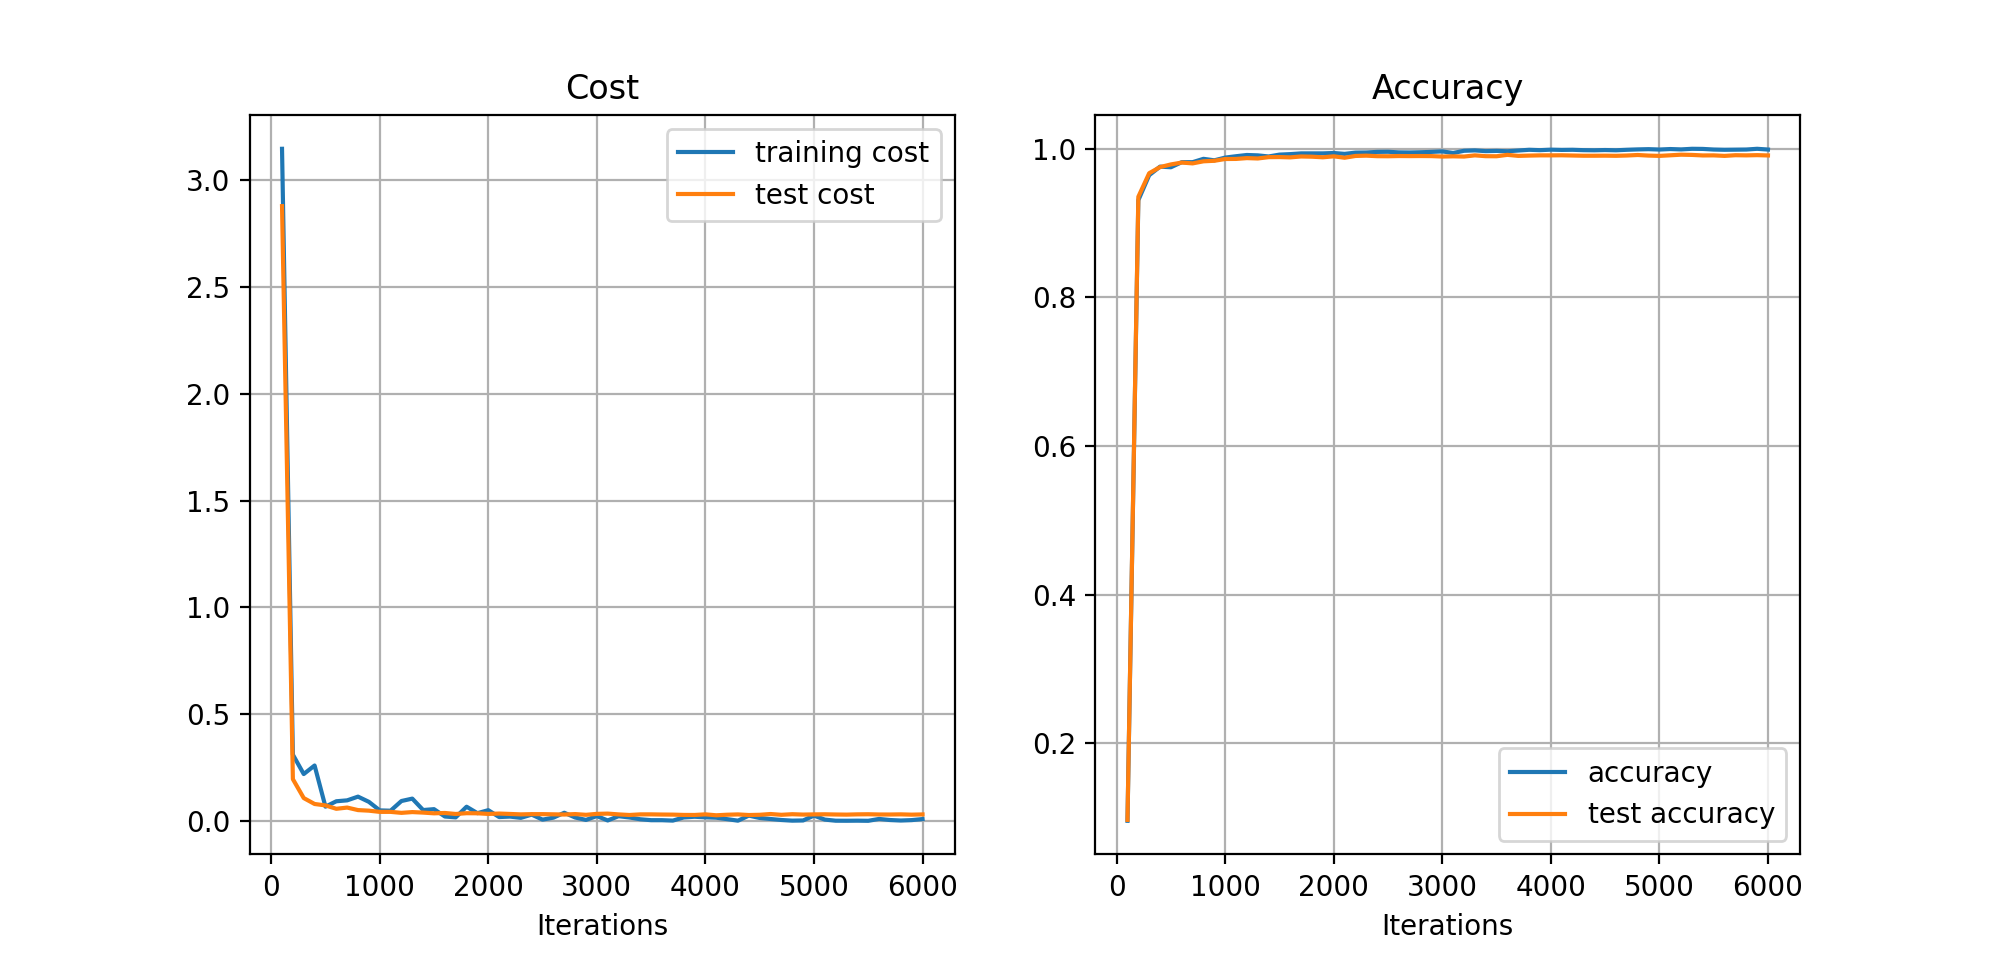
\includegraphics[width=120mm]{figures/assignment_3/improved_torch4.png}
\caption{Example of caption}
\label{fig:example}
\end{figure}

\begin{figure}[ht!]
\centering
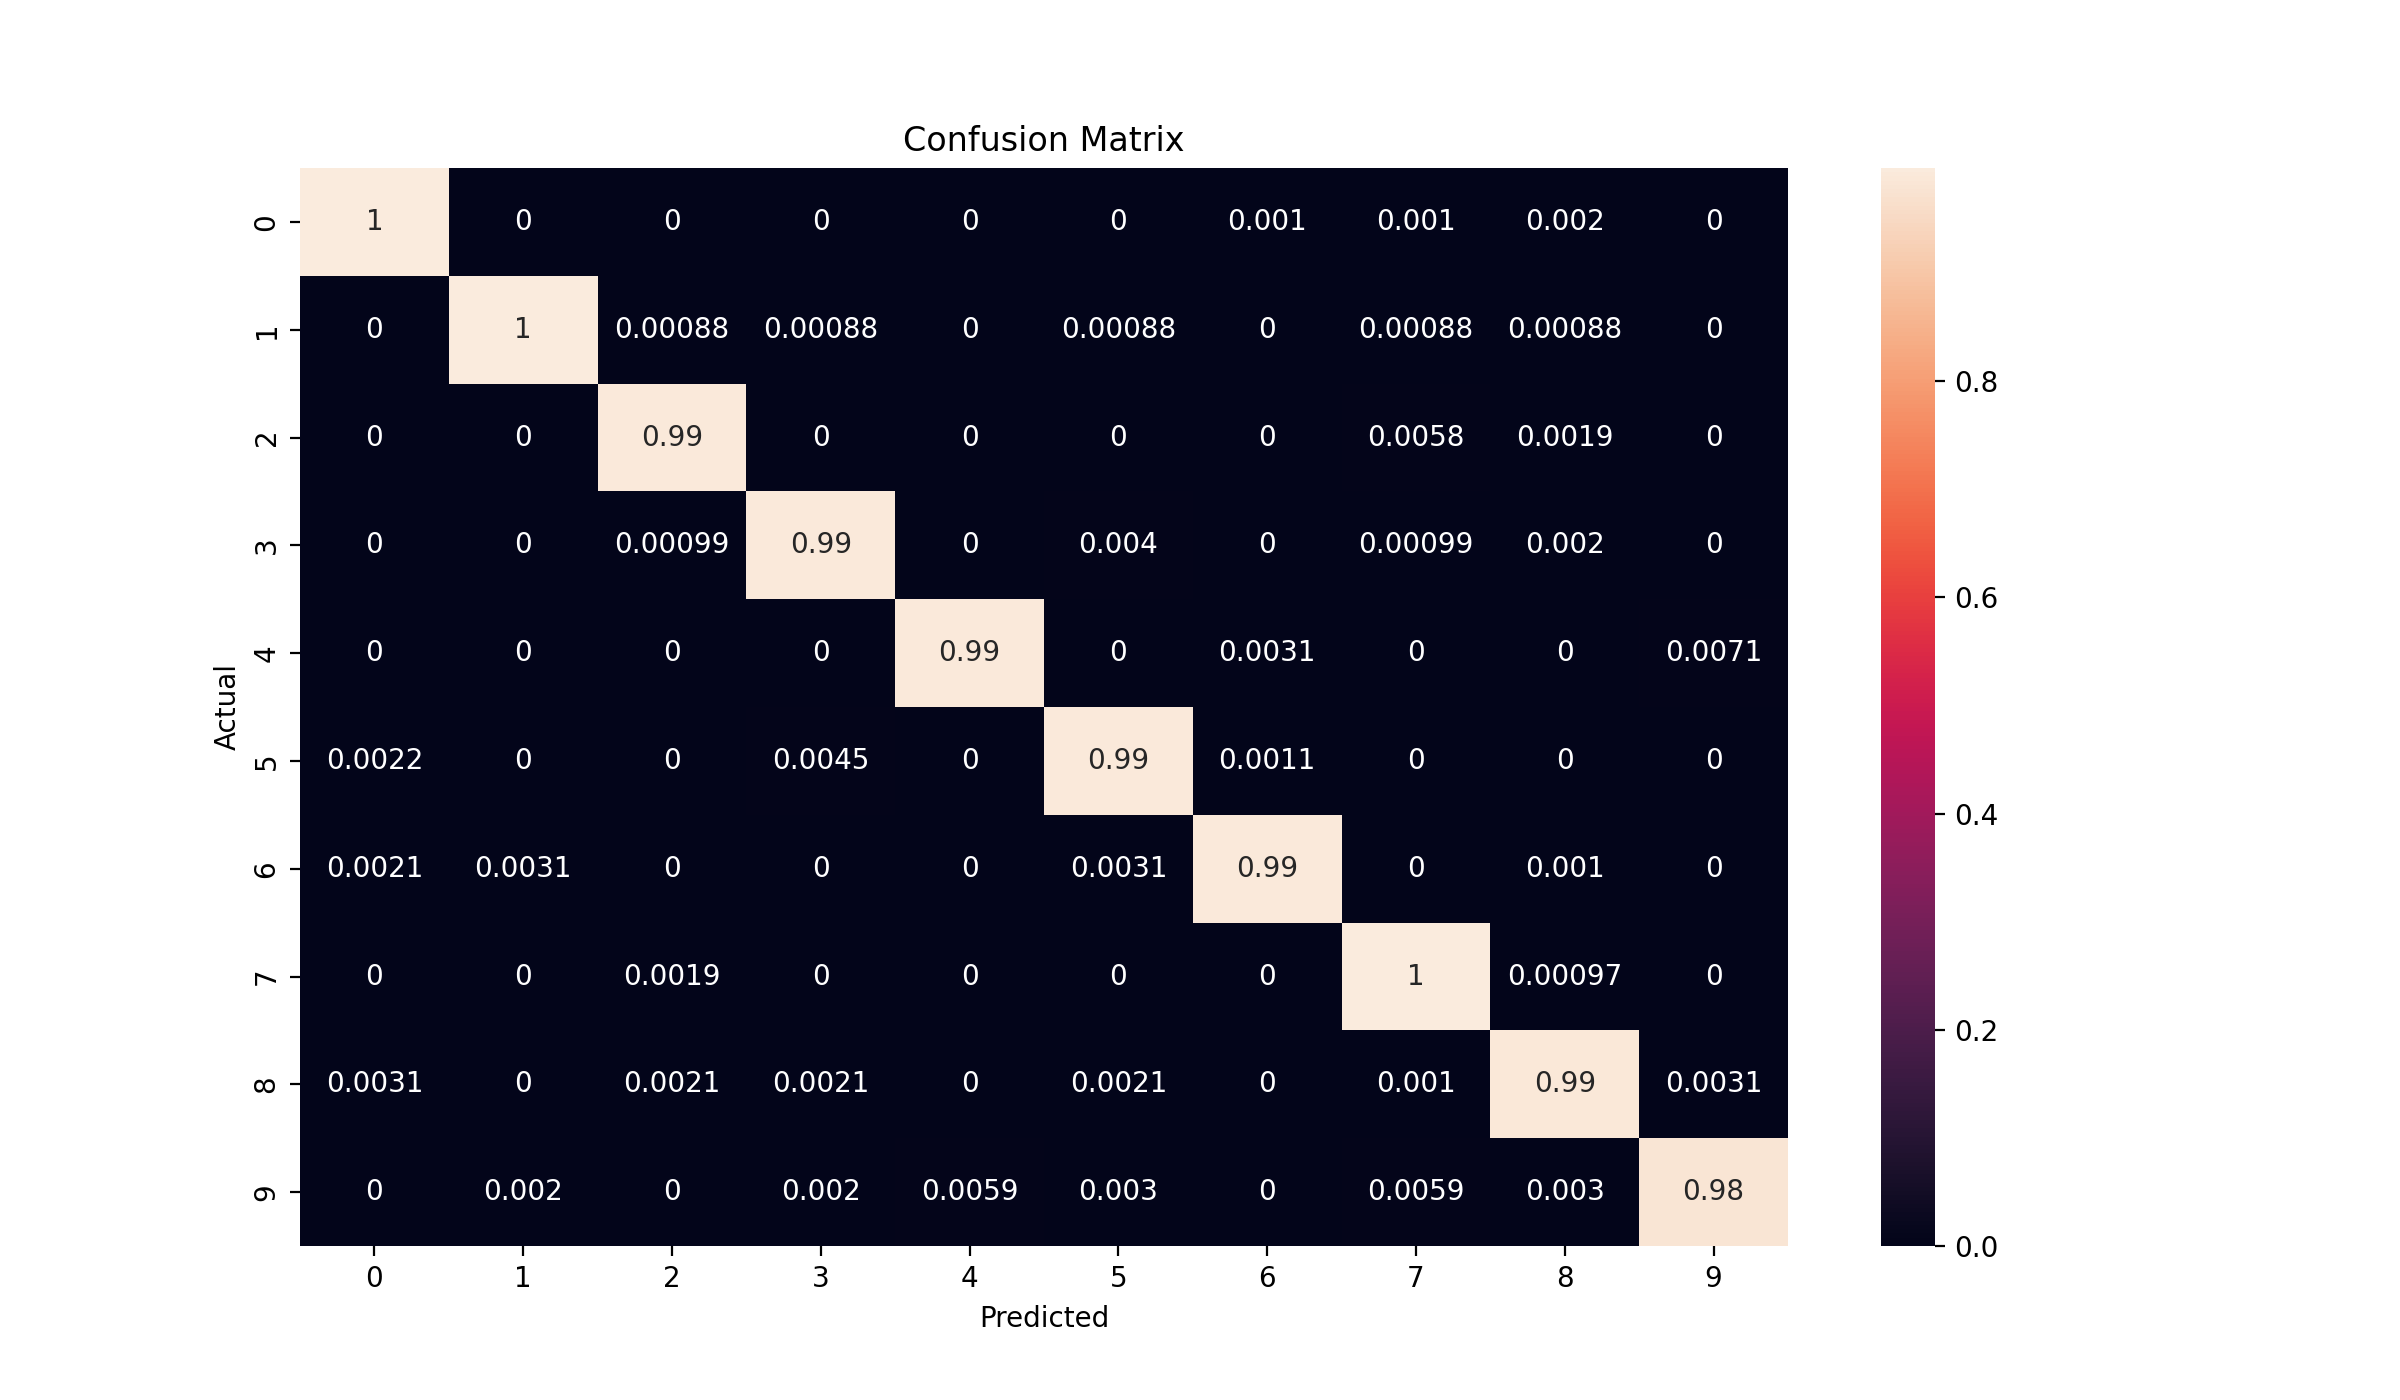
\includegraphics[width=120mm]{figures/assignment_3/improved_torch4_CM.png}
\caption{Example of caption}
\label{fig:example}
\end{figure}



\newpage
\section{Semantic segmentation of Biomedical images}

\textit{\textbf{Exercise 2.1}} Modifying our previous neural network by removing the fully connected layers replacing it with a 1 $\times$ 1 convolutional layer, we will now tackle a segmentation problem and evaluate it with Sørensen–Dice coefficient as performance measurement. In Figure: \ref{fig:segexample} we can see the result from the segmentation of a randomly picked test image. The segmentation models worst performance on the test set is presented in Figure: \ref{fig:worst}. Here we can see that it seems like the specimen is ending abrupt in the image, showing a lot of dark areas, presumably the background. Since this case is not well represented in the training set it is not so surprising that it performed badly on this image. 

\begin{figure}[ht!]
\centering
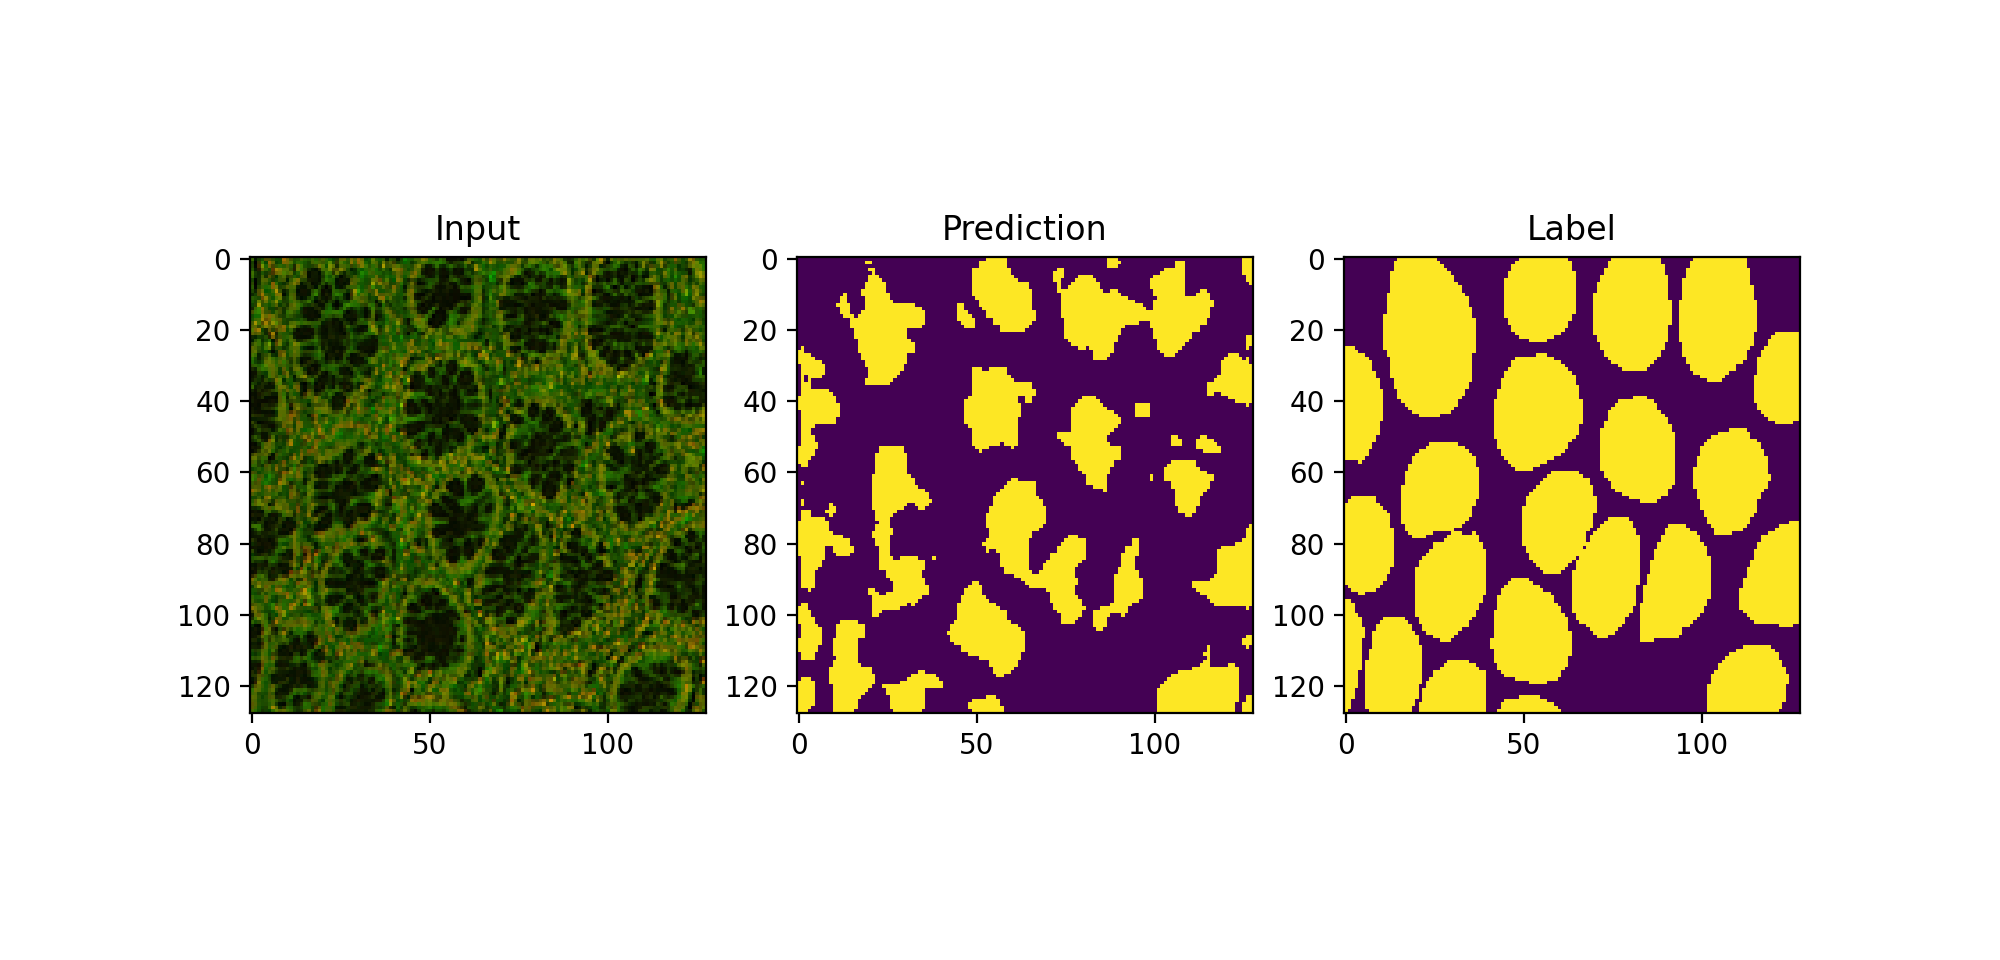
\includegraphics[width=100mm]{figures/assignment_3/segmentation_test4.png}
\caption{Segmentation of test-image: image\_05.png}
\label{fig:segexample}
\end{figure}

\begin{figure}[ht!]
\centering
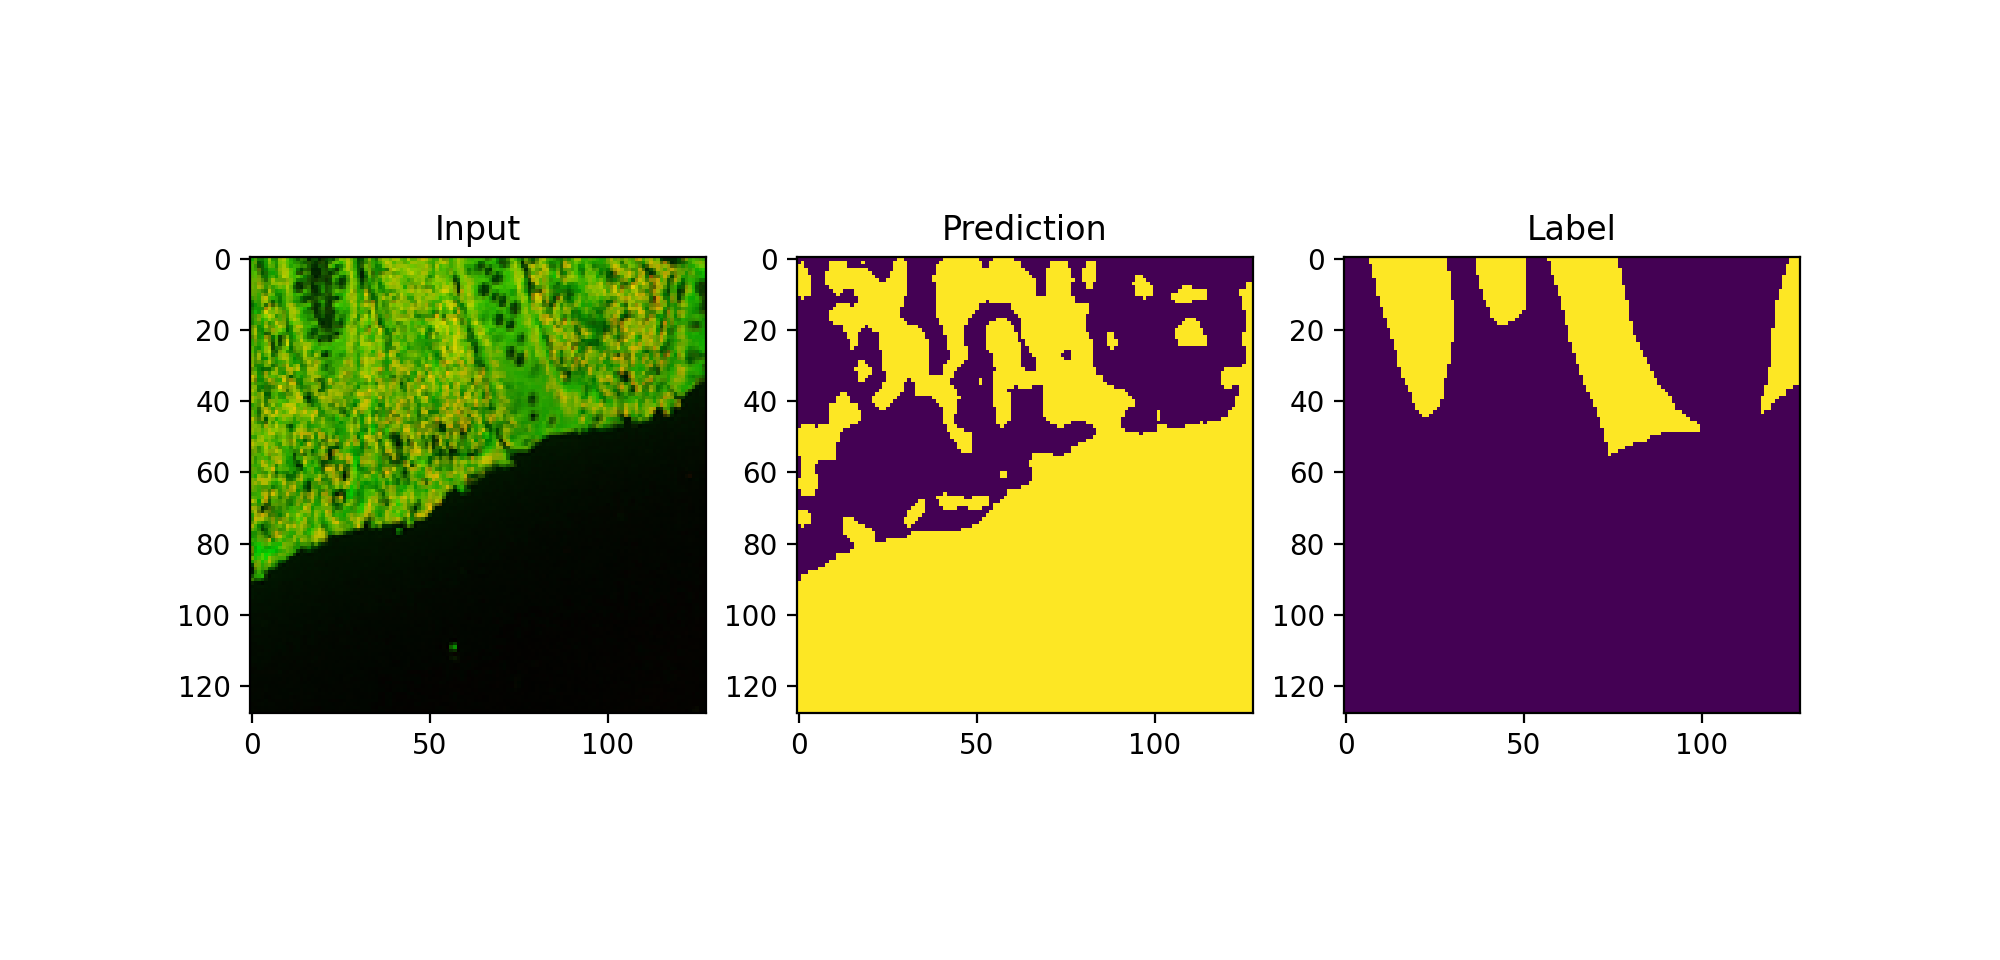
\includegraphics[width=100mm]{figures/assignment_3/segmentation_worst.png}
\caption{Segmentation of test-image: image\_11.png}
\label{fig:worst}
\end{figure}

\begin{table}[ht!]
\centering
\begin{tabular}{ll}\hline 
 \textbf{Hyperparameters}&    \\ \hline
 Epochs&  150 \\ 
 Optimizer& Adam  \\
 learning& 0.003 \\ \hline
\textbf{Result: }&   0.773\% \\ \hline
\end{tabular}
\caption{Hyperparameters Exercise 2.1}
\label{tab:tab8}
\end{table}

\textit{\textbf{Exercise 2.2}}
\textbf{Model 1: } Using batchnormalization 

\begin{table}[ht!]
\centering
\begin{tabular}{ll}\hline 
 \textbf{Hyperparameters}&    \\ \hline
 Epochs&  150 \\ 
 Optimizer& Adam  \\
 learning& 0.003 \\ \hline
\textbf{Result: }&   0.858\% \\ \hline
\end{tabular}
\caption{Hyperparameters Exercise 2.1, Model 1}
\label{tab:tab8}
\end{table}

\begin{thebibliography}{1}

\bibitem{Asimov} Asimov, Issac (1942). Runaround

\end{thebibliography}

\end{document}
